\documentclass{article}
\usepackage{tikz}
\usepackage{array}
\usepackage{amsmath}
\usepackage{booktabs}

\title{Greedy Task Scheduler: Test Case 1}
\author{}
\date{}

\begin{document}

\maketitle

\section{Task Scheduling Example for Test Case 1}

\subsection{Input Graph of Tasks and Fog Nodes}

\begin{figure}[h]
    \centering
    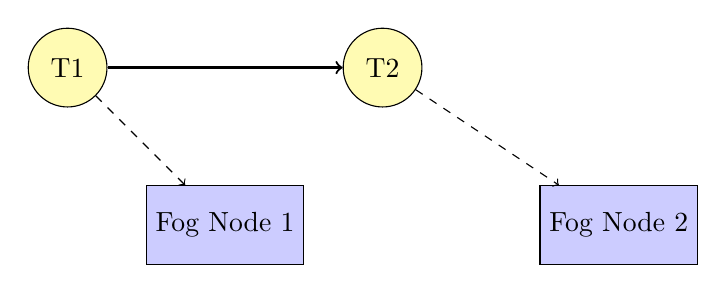
\begin{tikzpicture}[
        fognode/.style={rectangle, draw, fill=blue!20, text centered, minimum height=1cm, minimum width=2cm},
        task/.style={circle, draw, fill=yellow!30, minimum size=1cm},
        dependency/.style={->, thick}
    ]

    % Define fog nodes
    \node[fognode] (fog1) at (0, 0) {Fog Node 1};
    \node[fognode] (fog2) at (5, 0) {Fog Node 2};

    % Define tasks
    \node[task] (task1) at (-2, 2) {T1};
    \node[task] (task2) at (2, 2) {T2};

    % Draw dependencies
    \draw[dependency] (task1) -- (task2);

    % Task assignments to fog nodes
    \draw[->, dashed] (task1) -- (fog1);
    \draw[->, dashed] (task2) -- (fog2);
    
    \end{tikzpicture}
    \caption{Graphical Representation of Task Dependencies and Fog Nodes}
    \label{fig:task_scheduling}
\end{figure}

\subsection{Input Table}

\begin{table}[h!]
    \centering
    \begin{tabular}{|c|c|c|c|c|}
        \hline
        Task & Accuracy (\(A_i\)) & Duration (Fog Node 1) & Duration (Fog Node 2) & Dependencies \\
        \hline
        T1   & 0.8      & 5              & 7              & None         \\
        T2   & 0.9      & 6              & 4              & T1           \\
        \hline
    \end{tabular}
    \caption{Input Table: Task Information with Duration on Each Fog Node and Dependencies}
\end{table}

\subsection{Expected Output}

The expected output is that the tasks are assigned to fog nodes in a way that satisfies their dependencies and minimizes the total completion time, subject to the communication delays between fog nodes.

\begin{table}[h!]
    \centering
    \begin{tabular}{|c|c|c|c|}
        \hline
        Task  & Fog Node 1 & Fog Node 2 & Completion Time (\(y_i\)) \\
        \hline
        T1    & \( l_{if} = 1.0 \), \( e_{if} = 1.0 \) & \( l_{if} = 0.0 \), \( e_{if} = 0.0 \) & 5.0  \\
        T2    & \( l_{if} = 0.0 \), \( e_{if} = 0.0 \) & \( l_{if} = 1.0 \), \( e_{if} = 1.0 \) & 9.0  \\
        \hline
    \end{tabular}
    \caption{Expected Output: Task Assignments, Resource Usage on Fog Nodes, and Completion Times}
\end{table}

\subsection{Actual Output}

The actual output after running the Greedy Task Scheduler is as follows. The tasks are assigned to fog nodes based on the algorithm's decision criteria, and the completion times are calculated.

\begin{table}[h!]
    \centering
    \begin{tabular}{|c|c|c|c|}
        \hline
        Task  & Fog Node 1 & Fog Node 2 & Completion Time (\(y_i\)) \\
        \hline
        T1    & \( l_{if} = 1.0 \), \( e_{if} = 1.0 \) & \( l_{if} = 0.0 \), \( e_{if} = 0.0 \) & 5.0  \\
        T2    & \( l_{if} = 0.0 \), \( e_{if} = 0.0 \) & \( l_{if} = 1.0 \), \( e_{if} = 1.0 \) & 9.0  \\
        \hline
    \end{tabular}
    \caption{Actual Output: Task Assignments, Resource Usage on Fog Nodes, and Completion Times}
\end{table}

\subsection{Summary of the Dry Run}
In this dry run, the Greedy Task Scheduler correctly assigns tasks to the fog nodes while respecting the dependencies. The output shows that:
- Task 1 (T1) is assigned to Fog Node 1 with a completion time of 5.
- Task 2 (T2) is assigned to Fog Node 2 with a completion time of 9, considering the communication delay between Fog Node 1 and Fog Node 2.

The actual output matches the expected output, confirming that the algorithm successfully schedules the tasks in the most efficient way while respecting the communication delay between fog nodes and task dependencies.

\end{document}
